%18/03 - Carlos Aguirre B322
\chapter{Introducción y descripción de algunas redes reales}
Aunque lo vayamos a utilizar como sinónimos, un grafo y una red no es lo mismo; el grafo es la representación matemática de la red. En una red aleatoria, no hay que medir nada; si una red biológica sale aleatoria, se ha medido mal. Las redes biológicas son todas de mundo pequeño. Además, casi todas son libres de escala. 

\section{Qué es una red}
Una red es un conjunto de elementos (personas, ciudades, proteínas, especies animales, productos químicos, etc) de las cuales algunas están conectadas con otras y otras no. Se puede representar en bolas que se unen con líneas con otras líneas. Las bolitas se denominan como nodos. 

Las redes se estudian con NetworkX y Cytoscape.

\section{Algunos ejemplos de redes y algunas de sus propiedades}
\subsection{World Wide Web}
La World Wide Web es la mayor red para la cual existe información topológica. Los nodos de la red son los documentos, y las ramas son los enlaces (hyperlinks) entre documentos. El tamaño actual de esta red es de más de 1000 millones de nodos. Esta red es dirigida: la página A apunta a la página B, pero sin que la página B apunte a la página A. 
El grupo CAIDA se dedica a analizar la red. Esta red es enorme, pudiendo dibujar solo a un nivel muy alto.

La distribución del grado de las páginas web tiene una distribución libre de escala tanto en los enlaces de salida como en los enlaces de entrada. Esto es una distribución de probabilidad. Por ejemplo, en el queso de Gruyere, los agujeros son de distinto tamaño, los cuales tienen una distribución de tamaño. Se llama libre de escala porque se pueden encontrar diez veces más los agujeros de un tamaño mayor y diez veces menos los agujeros de tamaño pequeño. Así, no hay una escala fija de la distribución (no se puede representar con ninguna escala, ni logarítmica ni nada). Esto con el queso manchego no pasa. Si en la WWW vemos cuántas páginas web tienen 100 enlaces de salida, 10, 1000, etc, y se dibuja en escala logarítmica logarítmica, sale una recta. Esto pasa también con los enlaces de entrada. 

La distancia entre dos páginas de la WWW es pequeña (entre 11 y 16). Los nodos de la WWW están muy clusterizados.

La cola de la derecha parece que rompe la recta. Las redes libres de escala se pueden producir por muchas razones, pero al utilizar un proceso evolutivo en el que cada tiempo se generan nuevos nodos y tienen mayor preferencia para conectarse a otros nodos, e incluso pueden desaparecer algunos nodos antiguos. Esto produce las colas residuales.

\begin{figure}[h]
\centering
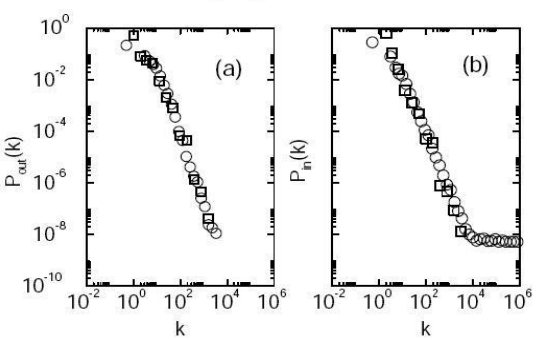
\includegraphics[width = 0.6\textwidth]{figs/www.png}
\end{figure}

Las redes libres de escala son muy resistentes a ataques aleatorios (fallos en la red) en cuanto a la conectividad, por lo que hay una razón evolutiva por la que las redes biológicas son libres de escala. La red regulatoria de P53 está muy estudiada y caracterizada. Uno de los elementos más importantes es MDM5.

\subsection{Internet}
Internet es la red de enlaces físicos entre ordenadores u otros servicios de comunicación. La topología de internet se suele estudiar a dos niveles: Enrutadores y Sistemas autónomos. Los enrutadores son las máquinas que mandan los "paquetes" a otros enrutadores. Hay algoritmos de enrutación que deciden hacia dónde enviar las cosas. Los sistemas autónomos son conjuntos de máquinas que organizan y gestionan otras máquinas.

Para ambos tipos de red (enrutadores y sistemas autónomos) el grado de cada nodo seguía una distribución libre de escala. De nuevo la red está altamente clusterizada (coeficiente de clustering entre 0,18 y 0,3) y los caminos entre nodos son cortos (aproximadamente 9). 

El \textbf{índice de clusterización} es una medida de la probabilidad de que los dos vecinos de un nodo sean vecinos entre sí, favoreciendo la creación de triángulos. Es decir, en redes sociales, que mis amigos también sean amigos entre sí. En biología, si dos proteínas son expresadas por una tercera proteína, las dos mantienen una relación entre sí (aunque puede no pasar). Los vecinos de un mismo nodo tienen una probabilidad alta de ser vecinos entre sí. En una red aleatoria, los vecinos de un nodo dependen de la probabilidad de rama de que esos nodos también sean vecinos entre sí (como cualquier otro).

La métrica de caminos cortos o largos se hace en comparación con el grafo aleatorio con el mismo número de nodos y ramas. En biología, los caminos también suelen ser cortos, y si son largos se puede deber a una enfermedad o patología.

\subsection{Red de actores}
Los nodos son actores, y dos de ellos están conectados si han participado juntos en alguna película. Actualmente, la red consta de unos 450.000 actores.
La distancia media entre actores es 3,65. La red está altamente clusterizada (100 veces más que un grafo aleatorio). La distribución de grados sigue una ley de potencias (libre de escala).

\subsection{Red de colaboración científica}
Los nodos están constituidos por científicos. Dos nodos están conectados si alguna vez publicaron un trabajo en común. La red de nuevo presenta una distribución libre de escala, caminos cortos entre los nodos y una alta clusterización. 

El \textbf{centro de la red} es el nodo que está a una menor distancia promedio del resto de nodos de la red. Este centro lo tiene un científico húngaro llamado Paul Erdös que trabajaba en teoría de grafos. 

Para una red de citaciones científicas, los nodos de la red son artículos científicos. Las ramas son citaciones entre artículos. Se tiene una base de datos de unos 750.000 artículos. Tanto los grados de entrada como los de salida siguen una distribución libre de escala.

\subsection{Red de contactos sexuales}
Los nodos y las ramas tienen una definición obvia. Tiene interés por la difusión de enfermedades (especialmente aquellas de transmisión sexual como el SIDA). Presenta una distribución libre de escala. Se sospecha que los datos de esta red no son totalmente fiables (es defectuosa al tener muchos datos falsos). Entre un 10-15\% es falsa.

Se define como k-core un grafo no dirigido creado a partir de un grafo más grande en el que se crean jerarquías o grupos en el que los nodos están separados por k vértices.

\subsection{Red de llamadas telefónicas}
Los nodos son números de teléfono. Las ramas son llamadas de larga distancia entre nodos. De nuevo la red presenta una distribución libre de escala.

\subsection{Redes lingüísticas}
Los nodos son palabras. Dos nodos están conectados si están juntas en alguna frase y hay solamente una palabra entre ambas. Un estudio realizado en inglés sobre 440.902 palabras presentó una distancia media de 2,62 y un índice de clusterización de 0,43.

Otra red linguística considera de nuevo los nodos como palabras. Dos nodos están conectados si se considera que ambas palabras son sinónimas (de acuerdo con el Merrian Webster Dictionary). El camino medio es de 4,7, el índice de clusterización es de 0,7 y los nodos presentan una distribución libre de escala.

En la red semántica, cada nodo es un objeto o un concepto. Dos nodos se relacionan entre sí, si existe una relación de la forma "es un" o "tiene un" entre ambos nodos. Se ha estudiado poco, pero parece presentar un camino medio corto, alta clusterización y una distribución de nodos libre de escala.

\subsection{Redes eléctricas}
La red eléctrica del Oeste de los Estados Unidos está compuesta por nodos (generadores, transformadores y subestaciones) y ramas (cables físicos entre nodos). La red tiene 4.941 nodos y un grado medio por nodo de 2,41. Esta red se aparta del patrón habitual teniendo una estructura muy jerárquita y en forma de estrella. Esto hace que sea muy frágil y condicionada a cuestiones económicas y políticas. Ocurre de forma similar con las redes de internet. No se utiliza el camino más rápido o corto, si no el camino más barato (como a la hora de buscar vuelos).

\section{Algunos ejemplos de redes biológicas y algunas de sus propiedades}
\subsection{Redes de ecología}
En las redes alimentarias, los nodos de la red son especies, y las ramas relaciones predador-presa entre especies. Las distancias son cortas entre los elementos de la red. En general, son redes con pocos nodos. 

Al ser redes pequeñas es difícil dibujar la distribución del grado de los nodos. Parecen presentar una distribución libre de escala, con un exponente inusualmente pequeño. Esta red es dirigida (aunque pueda haber dobles ramas). 

\subsection{Redes celulares}
Se presentan al estudiar el metabolismo de organismos. Los nodos son sustratos químicos (ATP, ADP, etc), y las ramas presentan reacciones químicas entre los sustratos. Esta red va de arriba a abajo, empezando con unos productos de entrada de la célula y terminando con productos de salida que la célula no puede descomponer más. 

\subsection{Redes neuronales}
Cada nodo es una neurona (biológica o artificial), y las ramas son conexiones sinápticas entre neuronas. La primera red estudiada de este tipo es la del gusano \textit{Caenorhabditis elegans}, del cual se tiene el mapa neuronal completo.

Las redes neuronales artificiales están ahora en auge para las inteligencias artificiales al utilizarse para el aprendizaje profundo.

\subsection{Redes de interacción de proteínas}
Cada nodo es una proteína. Las ramas representan relaciones de expresión entre las proteínas. Una de las redes más importantes es la red p53 de control de crecimiento del cáncer. Un paper muy bueno es \href{https://www.nature.com/articles/35042675}{Surfing the p53 network (DOI 10.1038/35042675)}.

Esta es la red en la que más se trabaja en biología. Se buscan los efectos entre los nodos (aumenta la expresión, inhibe), los componentes clave, los parámetros, etc. 

\subsection{Redes genéticas}
Cada nodo es expresión genética (nucleótidos). Las ramas conectan los nucleótidos que presentan un alto índice de similitud entre ambas. Una vez representada la red, se buscan familias o grupos de genes similares. Hay que diferenciar identidad con similitud (sobre todo con desajuste de fase). Se utiliza programación dinámica para calcular la mayor longitud de subsecuencia idéntica, como por ejemplo con el algoritmo Soldier's Walk. 

Si clusterizamos y obtenemos 2 cluster, cada cluster indica un gen con errores, o dos individuos distintos. Luego hay que interpretar por qué hay ese número de cluster. Normalmente hay muchos clusters que se quieren clasificar, y en cada cluster suele aparecer el mismo gen que se ha mutado. 

Las máquinas de microarrays ahora dan un conjunto de nucleótidos muy grandes, pero antes se obtenían fragmentos que había que unir. Para ello, se debían utilizar algoritmos sobre grafos para calcular cadenas largas a partir de las cadenas cortas, pero ahora ya no se usa por las mejoras tecnológicas. 
